\documentclass{exam}
\usepackage{graphicx}
\usepackage[utf8]{inputenc}
\usepackage[english]{babel}
\usepackage{amsmath}
\usepackage{hyperref}
\usepackage{amsthm}
\usepackage{tcolorbox}
\usepackage{amsfonts}
\usepackage{amssymb}
\usepackage{mathrsfs}
\usepackage{centernot}
\usepackage{cases}

\newcommand{\paren}[1]{\left(#1\right)}
\newcommand{\abs}[1]{\lvert#1\rvert}

\allowdisplaybreaks

\makeatletter
\long\def\paragraph{%
  \@startsection{paragraph}{4}%
  {\z@}{2ex \@plus 1ex \@minus .2ex}{-1em}%
  {\normalfont\normalsize\bfseries}%
}
\makeatother

\DeclareMathOperator{\lcm}{lcm}

\newbox\eeveebox
\setbox\eeveebox\hbox{
\raisebox{-2.5pt}{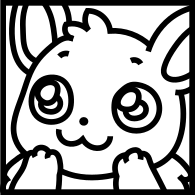
\includegraphics[height=2.5ex]{iibui.png}}}
\def\eeveeKawaii{\copy\eeveebox}

\newbox\skullbox
\setbox\skullbox\hbox{
\raisebox{-2.5pt}{
\includegraphics[height=2.5ex]{skull.png}}}
\def\bendingskull{\copy\skullbox}

\NewTColorBox{proposition}{m}{
  standard jigsaw,
  sharp corners,
  boxrule=0.4pt,
  coltitle=black,
  colframe=black,
  opacityback=0,
  opacitybacktitle=0,
  fonttitle=\normalfont\bfseries\upshape,
  fontupper=\normalfont,
  title={Proposition #1},
  after title={.},
  attach title to upper={\ },
}

\NewTColorBox{problem}{m}{
  standard jigsaw,
  sharp corners,
  boxrule=0.4pt,
  coltitle=black,
  colframe=black,
  opacityback=0,
  opacitybacktitle=0,
  fonttitle=\normalfont\bfseries\upshape,
  fontupper=\normalfont,
  title={Problem #1},
  after title={.},
  attach title to upper={\ },
}

\NewTColorBox{conjecture}{m}{
  standard jigsaw,
  sharp corners,
  boxrule=0.4pt,
  coltitle=black,
  colframe=black,
  opacityback=0,
  opacitybacktitle=0,
  fonttitle=\normalfont\bfseries\upshape,
  fontupper=\normalfont,
  title={Conjecture #1},
  after title={.},
  attach title to upper={\ },
}

\renewcommand\qedsymbol{$\eeveeKawaii$}

\title{Hammack Exercises - Part IV}
\author{FungusDesu}
\date{September 30th 2024}

\begin{document}

\maketitle

\section{Preface}
i dont really have anything to say

\section{Proofs}

\begin{problem}{12.2.4}
	A function $f:\mathbb Z\rightarrow\mathbb Z\times\mathbb Z$ is defined as $f(n)=(2n, n + 3)$. Verify whether this function is injective or surjective.
\end{problem}

The function $f$ is injective. To prove this, we shall show that $f(a) = f(b)$ implies $a = b$ for any integer $a,b$. Then we have the following system of equations 
\begin{align*}
	&\begin{cases}
		2a = 2b\\
		a + 3 = b + 3
	\end{cases}\\
	&\begin{cases}
		a = b\\
		a = b
	\end{cases}
\end{align*}

The function $f$ is not surjective, as there exists $(x, y) = (69, 420)\in\mathbb Z\times\mathbb Z$ for which $2n \neq 69$ for every $n\in\mathbb Z$, and so $(69, 420)$ is not in the image of $f$.

\begin{problem}{12.2.5}
	A function $f:\mathbb Z\rightarrow\mathbb Z$ is defined as $f(n)=2n+1$. Verify whether this function is injective or surjective.
\end{problem}

The function $f$ is injective. To see why, we show $f(a) = f(b)$ implies $a = b$ for any integer $a, b$. Then we have $2a + 1 = 2b + 1$ implies $a = b$.

The function $f$ is not surjective, since there does not exist $n\in\mathbb Z$ such that $2n + 1 = 420$.

\begin{problem}{12.2.6}
	A function $f:\mathbb Z\times\mathbb Z\rightarrow\mathbb Z$ is defined as $f(m, n)=3n-4m$. Verify whether this function is injective or surjective.
\end{problem}

The function $f$ is not injective, as there exist unequal elements $(0, 2)$ and $(3, 6)$ in $\mathbb Z\times\mathbb Z$ such that $f(0, 2) = f(3, 6) = 6$.

The function $f$ is surjective. To see why, consider an arbitrary integer $a$. We need to show that there exists $(m,n)\in\mathbb Z\times\mathbb Z$ such that $f(m, n) = 3n-4m = a$. By Proposition 7.1, there exists $m',n'\in\mathbb Z$ such that $3n'-4m'=\gcd(-4, 3) = 1$. Thus $3\cdot(an') - 4\cdot(am') = a$. Therefore for $m = am'$ and $n = an'$, we have $f(m,n) = a$.

\begin{problem}{12.2.7}
    A function $f:\mathbb Z\times\mathbb Z\rightarrow\mathbb Z$ is defined as $f(m, n)=2n-4m$. Verify whether this function is injective or surjective.
\end{problem}

The function $f$ is not injective, as there exist unequal elements $(0, 0)$ and $(1,2)$ in $\mathbb Z\times\mathbb Z$ such that $f(0, 0) = f(1, 2) = 0$.

The function $f$ is not surjective, as there does not exist $m, n\in\mathbb Z$ such that $f(m, n) = 2n - 4m = 1$ (the sum of two even numbers cannot be an odd number).

\begin{problem}{12.2.8}
    A function $f:\mathbb Z\times\mathbb Z\rightarrow \mathbb Z\times\mathbb Z$ is defined as $f(m,n)=(m+n, 2m + n)$. Verify whether this function is injective or surjective.
\end{problem}

The function $f$ is injective. To show why, we shall prove that $f(m, n) = f(m', n')$ implies $(m, n) = (m', n')$ for any $(m, n),(m',n')\in\mathbb Z^2$. Thus we have the following system of equations:
\begin{numcases}{}
    m + n = m' + n'\\
    2m + n = 2m' + n'
\end{numcases}
Subtracting equation $(1)$ from equation $(2)$ gives $m = m'$, and subsequently $n=n'$. Thus $(m, n) = (m',n')$.

The function $f$ is surjective. To show why, consider an arbitrary $(a, b) \in\mathbb Z\times\mathbb Z$. We shall show that there exists $(x, y) \in \mathbb Z\times\mathbb Z$ for which $f(x, y) = (a, b)$. Thus we have the following system of equations:
\begin{align*}
    \begin{cases}
        x + y = a\\
        2x + y = b
    \end{cases}\iff
    \begin{cases}
        x = b - a\\
        x + y = a
    \end{cases}\iff
    \begin{cases}
        x = b-a\\
        y = 2a - b
    \end{cases}
\end{align*}
Thus for any $(a, b)$, there exists $(x, y) = (b-a, 2a - b)$ such that $f(x, y) = (a, b)$.

\begin{problem}{12.2.9}
    Prove that the function $f:\mathbb R\setminus\{2\}\rightarrow\mathbb R\setminus\{5\}$ defined by $f(x)=\frac{5x-1}{x-2}$ is bijective.
\end{problem}

\begin{proof}
    We first show that $f$ is injective. To this end, we show that $f(a) = f(b)$ implies $a = b$ for any real number $a, b\neq 2$. Then
    \begin{align*}
        \frac{5a-1}{a-2} &= \frac{5b-1}{b-2}\\
        (5a-1)(b-2)&=(5b-1)(a-2)\\
        5ab - 10a - b + 2 &= 5ab - 10b - a + 2\\
        -10a + a &= -10b + b\\
        a &= b.
    \end{align*}
    We now show that $f$ is surjective. Consider an arbitrary element $y$ such that $y\in\mathbb R\setminus\{5\}$. We wish to prove there exists $x\in\mathbb R\setminus\{2\}$ for which $f(x) = y$. Then
    \begin{align*}
        \frac{5x-1}{x-2} = y \implies 5x-1 = xy-2y\implies x(5-y) = 1-2y\implies x = \frac{1-2y}{5-y}.
    \end{align*}
    And so $f(\frac{1-2y}{5-y}) = y$ for arbitrary $y\in\mathbb R\setminus\{5\}$. Since $f$ is both injective and surjective, it is also bijective.
\end{proof}

\begin{problem}{12.2.10}
    Prove the function $f:\mathbb R\setminus\{1\}\rightarrow\mathbb R\setminus\{1\}$ defined by $f(x)=\paren{\frac{x+1}{x-1}}^3$ is bijective.
\end{problem}

\begin{proof}
    We first show that $f$ is injective. To this end, we show that $f(a) = f(b)$ implies $a=b$ for any real number $a, b\neq1$. Note that the function $g:\mathbb R\rightarrow\mathbb R$ defined by $g(x) = x^3$ is injective. To show this, we prove that for $m,n\in\mathbb R$, we have $g(m) = g(n)$ implies $m = n$. Thus we have the following:
    \begin{align*}
        &m^3 = n^3\\
        \implies&(m-n)(m^2+mn+n^2) = 0\\
        \implies&(m-n)\paren{\paren{\frac m 2 + n}^2 + \frac{3m^2}4} = 0.
    \end{align*}
    If $m = n = 0$, then we are done. If $a\neq 0$ and $b\neq 0$, then we have $m-n = 0$ implies $m = n$. Using this fact and $f(a) = f(b)$, we deduce that
    \begin{align*}
        &\paren{\frac{a+1}{a-1}}^3 = \paren{\frac{b+1}{b-1}}^3\\
        \implies&\frac{a+1}{a-1} = \frac{b+1}{b-1}\\
        \implies&(a+1)(b-1) = (a-1)(b+1)\\
        \implies&ab-a+b-1 = ab+a-b-1\\
        \implies&a=b.
    \end{align*}

    We now show that $f$ is surjective. Consider an arbitrary element $y\in\mathbb R\setminus\{1\}$; we wish to show that there exists some $x\in\mathbb R\setminus\{1\}$ such that $f(x) = y$. Thus $x^3 = y$ implies $x=\sqrt[3]{y}$, which is the $x$ value we wish to find. Since $f$ is injective and surjective, it is also bijective.
\end{proof}

\begin{problem}{12.2.11}
    Consider the function $\theta:\{0,1\}\times\mathbb N\rightarrow\mathbb Z$ defined as $\theta(a, b)=(-1)^ab$. Is $\theta$ injective? Surjective? Bijective? Explain.
\end{problem}

The function $\theta$ is injective. To see why, we show that $\theta(x, y) = \theta(x', y')$ implies $(x, y) = (x', y')$. Then we have 
\begin{align*}
    (-1)^xy = (-1)^{x'}y'\\
    (-1)^{x-x'} = \frac{y}{y'}.
\end{align*}
Without loss of generality, assume $x = 0$ and $x' = 1$. Then $\frac{y}{y'}$. But since $y,y'\in\mathbb N$, this is not possible. Thus $x = x'$, which implies $y = y'$.

The function $\theta$ is not surjective, since there does not exist $a, b\in\{0, 1\}\times\mathbb N$ for which $(-1)^ab = 0$. Since $\theta$ is injective, but not surjective, it is not bijective.

\begin{problem}{12.2.12}
    Consider the function $\theta:\{0, 1\}\times\mathbb N\rightarrow\mathbb Z$ defined as $\theta(a,b)=a-2ab+b$. Is $\theta$ injective? Surjective? Bijective? Explain.
\end{problem}

The function $\theta$ is injective. To see why, we show that $\theta(x, y) = \theta(x', y')$ implies $(x, y) = (x', y')$. Then we have
\begin{align*}
    &x-2xy+y = x'-2x'y'+y'\\
    \implies&x(1-2y)+y = x'(1-2y') + y'.
\end{align*}
If $x=x'$, then it implies that $y=y'$. Without loss of generality, assume $x = 0$ and $x' = 1$, then it implies that $y = 1-y'$. The left hand side has a lower bound of 1, whereas the right hand side as an upper bound of 0; thus the equality does not hold for any $y, y'\in\mathbb N$. Thus $(x, y) = (x', y')$.

The function $\theta$ is surjective. To see why, we show that there exists some $(a, b)\in\{0, 1\}\times\mathbb N$ for which $\theta(a, b)\in\mathbb Z$. We have the following:
\begin{align}
    a-2ab+b = a(1-2b) + b.
\end{align}
If $a = 0$, then $(3) = b \ge 1$. If $a = 1$, then $(3)= 1 - b \le 0$. So there always exists some $(a, b)$ for which $\theta(a, b)\in\mathbb Z$. Since $\theta$ is injective and surjective, it is also bijective.

\begin{problem}{12.2.13}
    Consider the function $f:\mathbb R^2\rightarrow\mathbb R^2$ defined by the formula $f(x, y) = (xy, x^3)$. Is $f$ injective? Surjective? Bijective? Explain.
\end{problem}

The function $f$ is not injective, as there exist unequal elements $(0, 0)$ and $(0, 1)$ for which $f(0, 0) = f(0, 1) = (0, 0)$.

The function $f$ is not surjective, as there does not exists $(x, y)\in\mathbb R^2$ for which $f(x, y) = (-1, 0)$ ($(xy, x^3) = (0, 0)$ implies $x = 0$, and so $0y = 0$ for all real $y$). Since $f$ is not injective and not surjective, it is not bijective.

\begin{problem}{12.2.14}
    Consider the function $\theta:\mathscr P(\mathbb Z)\rightarrow\mathscr P(\mathbb Z)$ defined as $\theta(X) = \overline{X}$. Is $\theta$ injective? Surjective? Bijective? Explain.
\end{problem}

The function $\theta$ is injective. To see why, we shall show that $\theta(A) = \theta(B)$ implies $A = B$ for any $A, B\in\mathscr P(Z)$. Then
\begin{align*}
    \overline A = \overline B \implies \overline{\overline A} = \overline{\overline B} \implies A = B.
\end{align*}

The function $\theta$ is surjective. To see why, suppose an arbitrary set $Y\subseteq \mathbb Z$; we wish to show there exists some $X\subseteq\mathbb Z$ for which $\theta(X) = Y$. Then $\overline X = Y$ implies $X = \overline Y$, and so this is the set $X$ for which $\theta(X) = Y$.

\begin{problem}{12.2.18}
    Prove that the function $f:\mathbb N\rightarrow\mathbb Z$ defined as $f(n)=\frac{(-1)^n(2n-1)+1}4$ is bijective.
\end{problem}

\begin{proof}
    We first show that $f$ is injective. To this end, we show that $f(a) = f(b)$ implies $a = b$ for any natural $a, b$. Suppose $f(a) = f(b)$; then
    \begin{align*}
        \frac{(-1)^a(2a-1)+1}4 = \frac{(-1)^b(2b-1)+1}4 &\implies (-1)^a(2a-1) = (-1)^b(2b-1)\\
        &\implies\abs{(-1)^a(2a-1)} = \abs{(-1)^b(2b-1)}\\
        &\implies\abs{2a-1}=\abs{2b-1}
    \end{align*}
    Since $2a - 1$ and $2b - 1$ are always positive for natural $a, b$, it follows that
    \begin{align*}
        2a - 1 = 2b - 1 \implies a = b.
    \end{align*}

    We then show that $f$ is surjective. Consider an arbitrary element $y\in\mathbb Z$. We seek an $x\in\mathbb N$ for which $f(x) = y$, that is, for which
    \begin{align*}
        \frac{(-1)^x(2x-1) + 1}4 = y.
    \end{align*}
    If $y = 0$, then solving the equality gets $x=1$. If $y>0$, then $x = 2y\in\mathbb N$ is the solution to the equality. Observe that
    \begin{align*}
        f(2y) = \frac{(-1)^{2y}(4y-1) + 1}4 = y.
    \end{align*}
    If $y < 0$, then $x = -2y +1\in\mathbb N$ is the solution to the equality. Observe that
    \begin{align*}
        f(-2y + 1) = \frac{(-1)^{-2y+1}(2(-2y+1) - 1) + 1}4 = \frac{4y-2+1+1}4 = y.
    \end{align*}
    Thus for any $y\in\mathbb Z$, there exists $x\in\mathbb N$ such that $f(x) = y$, so $f$ is surjective. Since $f$ is both injective and surjective, it is also bijective.
\end{proof}
\newpage
\begin{problem}{12.3.1}
    Prove that if six integers are chosen at random, then at least two of them will have the same remainder when divided by $5$.
\end{problem}

\begin{proof}
    Let $X\subseteq\mathbb Z$ be the set of any six integers. Let $Y = \{0, 1, 2, 3, 4\}$ be the set of possible remainders an arbitrary integer can have when divided by $5$. Consider the function $$f:X\rightarrow Y,$$ where $f(x)$ is the remainder of $x$ when divided by $5$. As $\abs{X} = 6 > 5 = \abs{Y}$, it follows from the pigeonhole principle that $f$ is not injective. Thus there exists $a, b\in X$ for which $a\neq b$ such that $f(a) = f(b)$.
\end{proof}

\begin{proposition}{12.6.5}
    Consider a function $f:A\rightarrow B$ and a subset $X\subseteq A$. Then $X\subseteq f^{-1}(f(X))$.
\end{proposition}

\begin{proof}
    Suppose $x\in X$; then $f(x)\in f(X)$. Since $x\in X\subseteq A$, we have $x\in A$. By definition, the preimage of $f(X)$ is $f^{-1}(f(X)) = \{y\in A:f(y)\in f(X)\}$. Thus $x\in f^{-1}(f(X))$, and so $X\subseteq f^{-1}(f(X))$.
\end{proof}

\begin{conjecture}{12.6.6}
    Given a function $f:A\rightarrow B$ and a subset $Y\subseteq B$. Then $f(f^{-1}(Y))=Y$.
\end{conjecture}

\begin{proof}[Disproof]
    This conjecture is false due to the following counterexample. Let $f:\mathbb R\rightarrow\mathbb R$ defined by $f(x) = x^2$. Let $Y=\{-1, 1\}\in\mathbb R$. Note that $f(f^{-1}(Y)) = \{1\} \neq Y$, and we are done.
\end{proof}

\begin{problem}{13.2.1}
    Prove that $$\lim_{x\to5}(8x-3)=37.$$
\end{problem}

\begin{proof}
    Choose any $\varepsilon > 0$. Observe that
    \begin{align*}
        \abs{(8x - 3) - 37} = \abs{8(x - 5)} = 8\abs{x-5}.
    \end{align*}
    Choose $\delta = \frac{\varepsilon}8>0$, then $0 < \abs{x-5} < \delta$ yields $0 < 8\abs{x-5} = \abs{(8x-3)-37} < \frac{8\varepsilon}8 = \varepsilon$. Thus $$\lim_{x\to5}(8x-3) = 37.$$
\end{proof}

\begin{problem}{13.2.2}
    Prove that $$\lim_{x\to-1}(4x+6)=2.$$
\end{problem}

\begin{proof}
    Choose any $\varepsilon > 0$. Observe that
    \begin{align*}
        \abs{(4x+6)-2} = 4\abs{x-(-1)}.
    \end{align*}
    Choose $\delta = \frac{\varepsilon}4 > 0$, then $0 < \abs{x-(-1)} < \delta$ yields $0 < 4\abs{x-(-1)} = \abs{(4x+6)-2} < \frac{4\varepsilon}4 = \varepsilon$. Thus $$\lim_{x\to-1}(4x+6)=2.$$
\end{proof}

\begin{problem}{13.2.3}
    Prove that $$\lim_{x\to0}(x+2)=2.$$
\end{problem}

\begin{proof}
    Choose any $\varepsilon > 0$. Observe that
    \begin{align*}
        \abs{(x+2) - 2} = \abs{x - 0}.
    \end{align*}
    Choose $\delta=\varepsilon>0$. Then $0 < \abs{x - 0} < \delta$ yields $0 < \abs{x - 0} < \abs{x-0} = \abs{(x+2) - 2} < \varepsilon$. Thus $$\lim_{x\to0}(x+2)=2.$$
\end{proof}

\begin{problem}{13.2.4}
    Prove that $$\lim_{x\to8}(2x-7)=9.$$
\end{problem}

\begin{proof}
    Choose any $\varepsilon > 0$. Observe that $\abs{(2x - 7) - 9} = 2\abs{x-8}$. Choose $\delta = \frac{\varepsilon}2 > 0$. Suppose $0 < \abs{x - 8} < \delta$, then $0 < 2\abs{x-8} = \abs{(2x-7)-9} < \frac{2\varepsilon}2 = \varepsilon$. Thus $$\lim_{x\to8}(2x-7)=9.$$
\end{proof}

\end{document}
